\documentclass{article}
\usepackage[utf8]{inputenc}
\title{Lesson 20 - Discrete Mathematics}
\author{Matt Chung}
\date{April 01, 2018}
\usepackage{verbatim}
\usepackage{listings}
\usepackage{amsmath}
\usepackage{mathtools}
\usepackage{tikz}
\usetikzlibrary{calc}
\renewcommand{\thesubsection}{\thesection.\alph{subsection}}
\usepackage{indentfirst}

\begin{document}
\maketitle

\section{}

Adjacency matrix:

\[
\begin{bmatrix}
    0 & 0 & 1 & 1 & 0 \\
    0 & 0 & 0 & 1 & 1 \\
    1 & 0 & 0 & 0 & 1 \\
    1 & 1 & 0 & 0 & 1 \\
    0 & 1 & 1 & 1 & 0
\end{bmatrix}
\]

Incidence matrix:

\[
\begin{bmatrix}
    1 & 1 & 0 & 0 & 0 & 0 \\
    0 & 0 & 1 & 1 & 0 & 0 \\
    0 & 1 & 0 & 0 & 1 & 0 \\
    1 & 0 & 0 & 1 & 0 & 1 \\
    0 & 0 & 1 & 0 & 1 & 1 \\
\end{bmatrix}
\]

\section{}

\subsection{}

\textbf{Solution:} The Eulerian cycle is: $a, d, b, e, d, g, h, e, f, h, i, f, c, b, a$

\subsection{}

\textbf{Solution: } No hamiltonian cycle exists.

Since we are searching for a cycle, let's assume that we start on $a$ vertex. The next vertex in the cycle can be either $b$ or $d$. Let's choose $b$. Although there are three next vertices available, $b$ or $d$ or $e$, we know that we cannot choose $d$ because that's the vertex we must return to. Now that we're on $b$, we must select $c$ as the next vertex because if we were to choose $e$, the only path back to $c$ would be through $f$ and taking that path to $c$ would prevent us from moving in any direction. So, moving from $b$ to $c$, our next (and only available) vertex is $f$. From $f$, we have three options: $e$ or $h$ or $i$. We cannot choose $e$ because doing so would leave with only one path to $i$, from $h$. The same applies with moving from $f$ to $h$, we'd be stuck at $i$. So, the next vertex from $f$ is $i$. So, from $f$ to $i$, our only next option is $h$. Now that we're on $h$. However, from this point on, we are stuck since the penultimate vertex must be $d$, as stated above. Put differently, if we choose $g$ we cannot get to $e$ without first crossing over $d$, which we cannot do since $d$ needs to be the pentultimate vertex. The same applies to traveling from $h$ to $e$.

\section{}

\subsection{}

\textbf{Solution: } Bridges are: $\{\{a,b\}, \{c,d\}, \{e, f\}\}$

\subsection{}

\textbf{Solution: } Cutvertices are: $\{b, c, d, e\}$

\section{}

\subsection{}

\begin{center}
    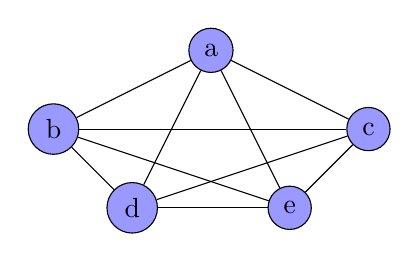
\begin{tikzpicture}
    \node[circle, fill=blue!40!white!, draw=black] (a) at (0,0) {a};
    
    \node[circle, fill=blue!40!white!, draw=black] (b) at ($(a) + (-2, -1)$) {b};
    
    \node[circle, fill=blue!40!white!, draw=black] (c) at ($(a) + (2, -1)$) {c};
    
    \node[circle, fill=blue!40!white!, draw=black] (d) at ($(a) + (-1, -2)$) {d};
    
    \node[circle, fill=blue!40!white!, draw=black] (e) at ($(a) + (1, -2)$) {e};
    
    \draw[-] (a) -- (b);
    \draw[-] (a) -- (c);
    \draw[-] (a) -- (d);
    \draw[-] (a) -- (e);
    
    \draw[-] (b) -- (c);
    \draw[-] (b) -- (d);
    \draw[-] (b) -- (e);
    
    \draw[-] (c) -- (d);
    \draw[-] (c) -- (e);
    
    \draw[-] (d) -- (e);
    
    \end{tikzpicture}
\end{center}

\subsection{}

No graph is possible, since there are more edges than there are vertices. More specifically, let's say that the vertex is $a$, the vertex with (supposedly) six edges. But since there are only five vertices in total, it's not possible for $a$ to form its final two edges.

\subsection{}

\begin{center}
    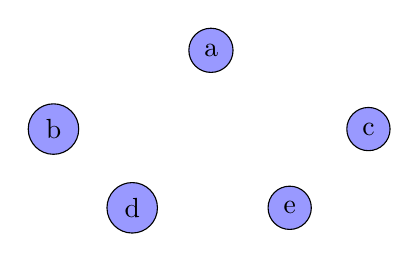
\begin{tikzpicture}
    \node[circle, fill=blue!40!white!, draw=black] (a) at (0,0) {a};
    
    \node[circle, fill=blue!40!white!, draw=black] (b) at ($(a) + (-2, -1)$) {b};
    
    \node[circle, fill=blue!40!white!, draw=black] (c) at ($(a) + (2, -1)$) {c};
    
    \node[circle, fill=blue!40!white!, draw=black] (d) at ($(a) + (-1, -2)$) {d};
    
    \node[circle, fill=blue!40!white!, draw=black] (e) at ($(a) + (1, -2)$) {e};
    
    \end{tikzpicture}
\end{center}

\subsection{}

\textbf{Solution: }

\begin{center}
    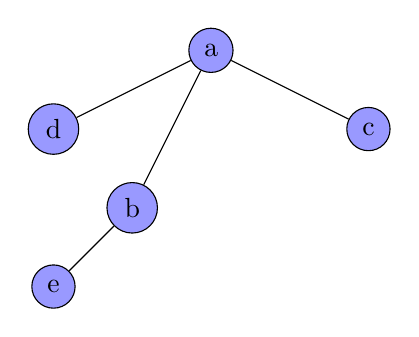
\begin{tikzpicture}
    \node[circle, fill=blue!40!white!, draw=black] (a) at (0,0) {a};
    
    \node[circle, fill=blue!40!white!, draw=black] (d) at ($(a) + (-2, -1)$) {d};
    
    \node[circle, fill=blue!40!white!, draw=black] (c) at ($(a) + (2, -1)$) {c};
    
    \node[circle, fill=blue!40!white!, draw=black] (b) at ($(a) + (-1, -2)$) {b};
    
    \node[circle, fill=blue!40!white!, draw=black] (e) at ($(b) + (-1, -1)$) {e};
    
    \draw[-] (a) -- (b);
    \draw[-] (a) -- (c);
    \draw[-] (a) -- (d);
    
    \draw[-] (b) -- (e);
    
    \end{tikzpicture}
\end{center}

\subsection{}

\begin{center}
    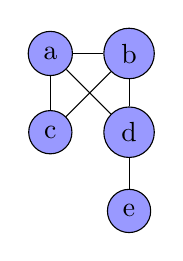
\begin{tikzpicture}
    \node[circle, fill=blue!40!white!, draw=black] (a) at (0,0) {a};
    
    \node[circle, fill=blue!40!white!, draw=black] (b) at (1,0) {b};
    
    \node[circle, fill=blue!40!white!, draw=black] (c) at ($(a) + (0, -1)$) {c};
    
    \node[circle, fill=blue!40!white!, draw=black] (d) at ($(b) + (0, -1)$) {d};
    
    \node[circle, fill=blue!40!white!, draw=black] (e) at ($(d) + (0, -1)$) {e};
    
    \draw[-] (a) -- (b);
    \draw[-] (a) -- (c);
    \draw[-] (a) -- (d);
    \draw[-] (b) -- (c);
    \draw[-] (b) -- (d);
    \draw[-] (d) -- (e);
    
    \end{tikzpicture}
\end{center}





\section{}
\textbf{Solution:} Total number of edges: $f - t$.

Let $f$ equal the number of vertices within a forest. Let $t$ equal the number of trees in the forest. From a theorem in a book, we know that a tree on $n$ has $n-1$ edges; simply put, there's one less edge for a given a number of vertices. In other words, the number of edges is one less for every additional tree.  Therefore, for a forest, with $t$ number of trees, we subtract simply subtract $t$, number of trees, to arrive at from $f$, the total number of vertices. $\clubsuit$

\newpage

\section{Bonus: }

\textbf{Solution: } 4 star-like, nonisomorphic trees

Based off of a definition of a star-like tree, only a single vertex can have more than two edges. Put differently, any tree where more than one vertex contains more than two edges is not considered star like. Therefore, only a tree's root can contain \textbf{more than} two edges. I emphasize \textbf{more than} because a root with only two edges would not be considered star-like. So, let's start with drawing the original six vertices star-like tree:

\begin{center}
    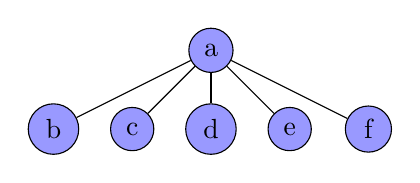
\begin{tikzpicture}
    \node[circle, fill=blue!40!white!, draw=black] (a) at (0,0) {a};
    
    \node[circle, fill=blue!40!white!, draw=black] (b) at ($(a) + (-2, -1)$) {b};
    
    \node[circle, fill=blue!40!white!, draw=black] (c) at ($(a) + (-1, -1)$) {c};
    
    \node[circle, fill=blue!40!white!, draw=black] (d) at ($(a) + (0, -1)$) {d};
    
    \node[circle, fill=blue!40!white!, draw=black] (e) at ($(a) + (1, -1)$) {e};
    
    \node[circle, fill=blue!40!white!, draw=black] (f) at ($(a) + (2, -1)$) {f};
    
    
    
    \draw[-] (a) -- (b);
    \draw[-] (a) -- (c);
    \draw[-] (a) -- (d);
    \draw[-] (a) -- (e);
    \draw[-] (a) -- (f);
    
    \end{tikzpicture}
\end{center}

Next, instead of drawing five direct children connected to the root, we draw only four. The sixth vertex is then connected to any one of the five children -- no difference to which child. In other words, connecting the sixth vertex to the fifth vertex and connecting the sixth vertex to the fourth vertex is isomorphic.

\begin{center}
    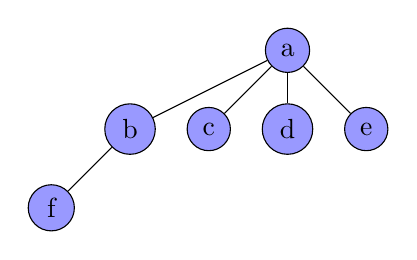
\begin{tikzpicture}
    \node[circle, fill=blue!40!white!, draw=black] (a) at (0,0) {a};
    
    \node[circle, fill=blue!40!white!, draw=black] (b) at ($(a) + (-2, -1)$) {b};
    
    \node[circle, fill=blue!40!white!, draw=black] (c) at ($(a) + (-1, -1)$) {c};
    
    \node[circle, fill=blue!40!white!, draw=black] (d) at ($(a) + (0, -1)$) {d};
    
    \node[circle, fill=blue!40!white!, draw=black] (e) at ($(a) + (1, -1)$) {e};
    
    \node[circle, fill=blue!40!white!, draw=black] (f) at ($(b) + (-1, -1)$) {f};
    
    
    
    \draw[-] (a) -- (b);
    \draw[-] (a) -- (c);
    \draw[-] (a) -- (d);
    \draw[-] (a) -- (e);
    \draw[-] (b) -- (f);
    
    \end{tikzpicture}
\end{center}

\begin{center}
    \begin{tikzpicture}
    \node[circle, fill=blue!40!white!, draw=black] (a) at (0,0) {a};
    
    \node[circle, fill=blue!40!white!, draw=black] (b) at ($(a) + (-2, -1)$) {b};
    
    \node[circle, fill=blue!40!white!, draw=black] (c) at ($(a) + (-1, -1)$) {c};
    
    \node[circle, fill=blue!40!white!, draw=black] (d) at ($(a) + (0, -1)$) {d};
    
    \node[circle, fill=blue!40!white!, draw=black] (e) at ($(f) + (-1, -1)$) {e};
    
    \node[circle, fill=blue!40!white!, draw=black] (f) at ($(b) + (-1, -1)$) {f};
    
    
    
    \draw[-] (a) -- (b);
    \draw[-] (a) -- (c);
    \draw[-] (a) -- (d);
    \draw[-] (e) -- (f);
    \draw[-] (b) -- (f);
    
    \end{tikzpicture}
\end{center}

\begin{center}
    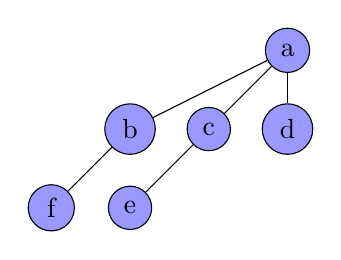
\begin{tikzpicture}
    \node[circle, fill=blue!40!white!, draw=black] (a) at (0,0) {a};
    
    \node[circle, fill=blue!40!white!, draw=black] (b) at ($(a) + (-2, -1)$) {b};
    
    \node[circle, fill=blue!40!white!, draw=black] (c) at ($(a) + (-1, -1)$) {c};
    
    \node[circle, fill=blue!40!white!, draw=black] (d) at ($(a) + (0, -1)$) {d};
    
    \node[circle, fill=blue!40!white!, draw=black] (e) at ($(c) + (-1, -1)$) {e};
    
    \node[circle, fill=blue!40!white!, draw=black] (f) at ($(b) + (-1, -1)$) {f};
    
    
    
    \draw[-] (a) -- (b);
    \draw[-] (a) -- (c);
    \draw[-] (a) -- (d);
    \draw[-] (e) -- (c);
    \draw[-] (b) -- (f);
    
    \end{tikzpicture}
\end{center}


\end{document}